%
% This is an example LaTeX file which uses the SANDreport class file.
% It shows how a SAND report should be formatted, what sections and
% elements it should contain, and how to use the SANDreport class.
% It uses the LaTeX article class, but not the strict option.
% ItINLreport uses .eps logos and files to show how pdflatex can be used
%
% Get the latest version of the class file and more at
%    http://www.cs.sandia.gov/~rolf/SANDreport
%
% This file and the SANDreport.cls file are based on information
% contained in "Guide to Preparing {SAND} Reports", Sand98-0730, edited
% by Tamara K. Locke, and the newer "Guide to Preparing SAND Reports and
% Other Communication Products", SAND2002-2068P.
% Please send corrections and suggestions for improvements to
% Rolf Riesen, Org. 9223, MS 1110, rolf@cs.sandia.gov
%
\documentclass[pdf,12pt]{INLreport}
% pslatex is really old (1994).  It attempts to merge the times and mathptm packages.
% My opinion is that it produces a really bad looking math font.  So why are we using it?
% If you just want to change the text font, you should just \usepackage{times}.
% \usepackage{pslatex}
\usepackage{times}
\usepackage{longtable}
\usepackage[FIGBOTCAP,normal,bf,tight]{subfigure}
\usepackage{amsmath}
\usepackage{amssymb}
\usepackage[labelfont=bf]{caption}
\usepackage{pifont}
\usepackage{enumerate}
\usepackage{listings}
\usepackage{fullpage}
\usepackage{xcolor}          % Using xcolor for more robust color specification
\usepackage{ifthen}          % For simple checking in newcommand blocks
\usepackage{textcomp}
%\usepackage{authblk}         % For making the author list look prettier
%\renewcommand\Authsep{,~\,}

% Custom colors
\definecolor{deepblue}{rgb}{0,0,0.5}
\definecolor{deepred}{rgb}{0.6,0,0}
\definecolor{deepgreen}{rgb}{0,0.5,0}
\definecolor{forestgreen}{RGB}{34,139,34}
\definecolor{orangered}{RGB}{239,134,64}
\definecolor{darkblue}{rgb}{0.0,0.0,0.6}
\definecolor{gray}{rgb}{0.4,0.4,0.4}

\lstset {
  basicstyle=\ttfamily,
  frame=single
}

\setcounter{secnumdepth}{5}
\lstdefinestyle{XML} {
    language=XML,
    extendedchars=true,
    breaklines=true,
    breakatwhitespace=true,
%    emph={name,dim,interactive,overwrite},
    emphstyle=\color{red},
    basicstyle=\ttfamily,
%    columns=fullflexible,
    commentstyle=\color{gray}\upshape,
    morestring=[b]",
    morecomment=[s]{<?}{?>},
    morecomment=[s][\color{forestgreen}]{<!--}{-->},
    keywordstyle=\color{cyan},
    stringstyle=\ttfamily\color{black},
    tagstyle=\color{darkblue}\bf\ttfamily,
    morekeywords={name,type},
%    morekeywords={name,attribute,source,variables,version,type,release,x,z,y,xlabel,ylabel,how,text,param1,param2,color,label},
}
\lstset{language=python,upquote=true}

\usepackage{titlesec}
\newcommand{\sectionbreak}{\clearpage}
\setcounter{secnumdepth}{4}

%\titleformat{\paragraph}
%{\normalfont\normalsize\bfseries}{\theparagraph}{1em}{}
%\titlespacing*{\paragraph}
%{0pt}{3.25ex plus 1ex minus .2ex}{1.5ex plus .2ex}

%%%%%%%% Begin comands definition to input python code into document
\usepackage[utf8]{inputenc}

% Default fixed font does not support bold face
\DeclareFixedFont{\ttb}{T1}{txtt}{bx}{n}{9} % for bold
\DeclareFixedFont{\ttm}{T1}{txtt}{m}{n}{9}  % for normal

\usepackage{listings}

% Python style for highlighting
\newcommand\pythonstyle{\lstset{
language=Python,
basicstyle=\ttm,
otherkeywords={self, none, return},             % Add keywords here
keywordstyle=\ttb\color{deepblue},
emph={MyClass,__init__},          % Custom highlighting
emphstyle=\ttb\color{deepred},    % Custom highlighting style
stringstyle=\color{deepgreen},
frame=tb,                         % Any extra options here
showstringspaces=false            %
}}


% Python environment
\lstnewenvironment{python}[1][]
{
\pythonstyle
\lstset{#1}
}
{}

% Python for external files
\newcommand\pythonexternal[2][]{{
\pythonstyle
\lstinputlisting[#1]{#2}}}

\lstnewenvironment{xml}
{}
{}

% Python for inline
\newcommand\pythoninline[1]{{\pythonstyle\lstinline!#1!}}

% Named Colors for the comments below (Attempted to match git symbol colors)
\definecolor{RScolor}{HTML}{8EB361}  % Sonat (adjusted for clarity)
\definecolor{DPMcolor}{HTML}{E28B8D} % Dan
\definecolor{JCcolor}{HTML}{82A8D9}  % Josh (adjusted for clarity)
\definecolor{AAcolor}{HTML}{8D7F44}  % Andrea
\definecolor{CRcolor}{HTML}{AC39CE}  % Cristian
\definecolor{RKcolor}{HTML}{3ECC8D}  % Bob (adjusted for clarity)
\definecolor{DMcolor}{HTML}{276605}  % Diego (adjusted for clarity)
\definecolor{PTcolor}{HTML}{990000}  % Paul

\def\DRAFT{} % Uncomment this if you want to see the notes people have been adding
% Comment command for developers (Should only be used under active development)
\ifdefined\DRAFT
  \newcommand{\nameLabeler}[3]{\textcolor{#2}{[[#1: #3]]}}
\else
  \newcommand{\nameLabeler}[3]{}
\fi
\newcommand{\alfoa}[1] {\nameLabeler{Andrea}{AAcolor}{#1}}
\newcommand{\cristr}[1] {\nameLabeler{Cristian}{CRcolor}{#1}}
\newcommand{\mandd}[1] {\nameLabeler{Diego}{DMcolor}{#1}}
\newcommand{\maljdan}[1] {\nameLabeler{Dan}{DPMcolor}{#1}}
\newcommand{\cogljj}[1] {\nameLabeler{Josh}{JCcolor}{#1}}
\newcommand{\bobk}[1] {\nameLabeler{Bob}{RKcolor}{#1}}
\newcommand{\senrs}[1] {\nameLabeler{Sonat}{RScolor}{#1}}
\newcommand{\talbpaul}[1] {\nameLabeler{Paul}{PTcolor}{#1}}
% Commands for making the LaTeX a bit more uniform and cleaner
\newcommand{\TODO}[1]    {\textcolor{red}{\textit{(#1)}}}
\newcommand{\xmlAttrRequired}[1] {\textcolor{red}{\textbf{\texttt{#1}}}}
\newcommand{\xmlAttr}[1] {\textcolor{cyan}{\textbf{\texttt{#1}}}}
\newcommand{\xmlNodeRequired}[1] {\textcolor{deepblue}{\textbf{\texttt{<#1>}}}}
\newcommand{\xmlNode}[1] {\textcolor{darkblue}{\textbf{\texttt{<#1>}}}}
\newcommand{\xmlString}[1] {\textcolor{black}{\textbf{\texttt{'#1'}}}}
\newcommand{\xmlDesc}[1] {\textbf{\textit{#1}}} % Maybe a misnomer, but I am
                                                % using this to detail the data
                                                % type and necessity of an XML
                                                % node or attribute,
                                                % xmlDesc = XML description
\newcommand{\default}[1]{~\\*\textit{Default: #1}}
\newcommand{\nb} {\textcolor{deepgreen}{\textbf{~Note:}}~}

%%%%%%%% End comands definition to input python code into document

%\usepackage[dvips,light,first,bottomafter]{draftcopy}
%\draftcopyName{Sample, contains no OUO}{70}
%\draftcopyName{Draft}{300}

% The bm package provides \bm for bold math fonts.  Apparently
% \boldsymbol, which I used to always use, is now considered
% obsolete.  Also, \boldsymbol doesn't even seem to work with
% the fonts used in this particular document...
\usepackage{bm}

% Define tensors to be in bold math font.
\newcommand{\tensor}[1]{{\bm{#1}}}

% Override the formatting used by \vec.  Instead of a little arrow
% over the letter, this creates a bold character.
\renewcommand{\vec}{\bm}

% Define unit vector notation.  If you don't override the
% behavior of \vec, you probably want to use the second one.
\newcommand{\unit}[1]{\hat{\bm{#1}}}
% \newcommand{\unit}[1]{\hat{#1}}

% Use this to refer to a single component of a unit vector.
\newcommand{\scalarunit}[1]{\hat{#1}}

% \toprule, \midrule, \bottomrule for tables
\usepackage{booktabs}

% \llbracket, \rrbracket
\usepackage{stmaryrd}

\usepackage{hyperref}
\hypersetup{
    colorlinks,
    citecolor=black,
    filecolor=black,
    linkcolor=black,
    urlcolor=black
}

\newcommand{\wiki}{\href{https://github.com/idaholab/raven/wiki}{RAVEN wiki}}

% Compress lists of citations like [33,34,35,36,37] to [33-37]
\usepackage{cite}

% If you want to relax some of the SAND98-0730 requirements, use the "relax"
% option. It adds spaces and boldface in the table of contents, and does not
% force the page layout sizes.
% e.g. \documentclass[relax,12pt]{SANDreport}
%
% You can also use the "strict" option, which applies even more of the
% SAND98-0730 guidelines. It gets rid of section numbers which are often
% useful; e.g. \documentclass[strict]{SANDreport}

% The INLreport class uses \flushbottom formatting by default (since
% it's intended to be two-sided document).  \flushbottom causes
% additional space to be inserted both before and after paragraphs so
% that no matter how much text is actually available, it fills up the
% page from top to bottom.  My feeling is that \raggedbottom looks much
% better, primarily because most people will view the report
% electronically and not in a two-sided printed format where some argue
% \raggedbottom looks worse.  If we really want to have the original
% behavior, we can comment out this line...
\raggedbottom
\setcounter{secnumdepth}{5} % show 5 levels of subsection
\setcounter{tocdepth}{5} % include 5 levels of subsection in table of contents

% ---------------------------------------------------------------------------- %
%
% Set the title, author, and date
%
\title{CashFlow Software Design Description}
%\author{%
%\begin{tabular}{c} Author 1 \\ University1 \\ Mail1 \\ \\
%Author 3 \\ University3 \\ Mail3 \end{tabular} \and
%\begin{tabular}{c} Author 2 \\ University2 \\ Mail2 \\ \\
%Author 4 \\ University4 \\ Mail4\\
%\end{tabular} }


\author{Andrea Alfonsi, Aaron Epiney, Paul Talbot, Cristian Rabiti}
 

% There is a "Printed" date on the title page of a SAND report, so
% the generic \date should [WorkingDir:]generally be empty.
\date{}


% ---------------------------------------------------------------------------- %
% Set some things we need for SAND reports. These are mandatory
%
\SANDnum{SDD-XXX}
\SANDprintDate{\today}
\SANDauthor{Andrea Alfonsi, Aaron Epiney, Paul Talbot, Cristian Rabiti}
\SANDreleaseType{Revision DRAFT}

% ---------------------------------------------------------------------------- %
% Include the markings required for your SAND report. The default is "Unlimited
% Release". You may have to edit the file included here, or create your own
% (see the examples provided).
%
% \include{MarkOUO} % Not needed for unlimted release reports

\def\component#1{\texttt{#1}}

% ---------------------------------------------------------------------------- %
\newcommand{\systemtau}{\tensor{\tau}_{\!\text{SUPG}}}

% Added by Sonat
\usepackage{placeins}
\usepackage{array}

\newcolumntype{L}[1]{>{\raggedright\let\newline\\\arraybackslash\hspace{0pt}}m{#1}}
\newcolumntype{C}[1]{>{\centering\let\newline\\\arraybackslash\hspace{0pt}}m{#1}}
\newcolumntype{R}[1]{>{\raggedleft\let\newline\\\arraybackslash\hspace{0pt}}m{#1}}

% end added by Sonat
% ---------------------------------------------------------------------------- %
%
% Start the document
%

\begin{document}
    \maketitle

    % ------------------------------------------------------------------------ %
    % An Abstract is required for SAND reports
    %
%    \begin{abstract}
%    \input abstract
%    \end{abstract}


    % ------------------------------------------------------------------------ %
    % An Acknowledgement section is optional but important, if someone made
    % contributions or helped beyond the normal part of a work assignment.
    % Use \section* since we don't want it in the table of context
    %
%    \clearpage
%    \section*{Acknowledgment}



%	The format of this report is based on information found
%	in~\cite{Sand98-0730}.


    % ------------------------------------------------------------------------ %
    % The table of contents and list of figures and tables
    % Comment out \listoffigures and \listoftables if there are no
    % figures or tables. Make sure this starts on an odd numbered page
    %
    \cleardoublepage		% TOC needs to start on an odd page
    \tableofcontents
    %\listoffigures
    %\listoftables


    % ---------------------------------------------------------------------- %
    % An optional preface or Foreword
%    \clearpage
%    \section*{Preface}
%    \addcontentsline{toc}{section}{Preface}
%	Although muggles usually have only limited experience with
%	magic, and many even dispute its existence, it is worthwhile
%	to be open minded and explore the possibilities.


    % ---------------------------------------------------------------------- %
    % An optional executive summary
    %\clearpage
    %\section*{Summary}
    %\addcontentsline{toc}{section}{Summary}
    %\input{Summary.tex}
%	Once a certain level of mistrust and skepticism has
%	been overcome, magic finds many uses in todays science



%	and engineering. In this report we explain some of the
%	fundamental spells and instruments of magic and wizardry. We
%	then conclude with a few examples on how they can be used
%	in daily activities at national Laboratories.


    % ---------------------------------------------------------------------- %
    % An optional glossary. We don't want it to be numbered
%    \clearpage
%    \section*{Nomenclature}
%    \addcontentsline{toc}{section}{Nomenclature}
%    \begin{description}
%          \item[alohomoral]
%           spell to open locked doors and containers
%          \item[leviosa]
%           spell to levitate objects
%    \item[remembrall]
%           device to alert you that you have forgotten something
%    \item[wand]
%           device to execute spells
%    \end{description}


    % ---------------------------------------------------------------------- %
    % This is where the body of the report begins; usually with an Introduction
    %
    \SANDmain		% Start the main part of the report

\section{Introduction}
\subsection{System Purpose}

The \textbf{\textit{CashFlow}} plug-in is a generalized module for economic analysis within RAVEN.
\\RAVEN is a flexible and multi-purpose uncertainty quantification (UQ), regression analysis, probabilistic risk assessment 
(PRA), data analysis and model optimization software.  Depending on the tasks to be accomplished and on the 
probabilistic
 characterization of the problem, RAVEN perturbs (Monte-Carlo, Latin hyper-cube, reliability surface search, etc.) the
 response of the system under consideration by altering its own parameters. 
 The data generated by the sampling process is analyzed using classical statistical
 and more advanced data mining approaches. RAVEN also manages the parallel dispatching (i.e. both on
 desktop/workstation and large High-Performance Computing machines) of the software representing the physical 
 model.
 For more information about the RAVEN software, see ~\cite{RAVENuserManual} and the RAVEN website (\url{raven.inl.gov}
\\The  \textbf{\textit{CashFlow}} module is a dedicated module of RAVEN and one of the first developed RAVEN plug-ins. 
A RAVEN plug-in is a software/module/library that has been developed to be linked to RAVEN at run-time, using the RAVEN APIs.


\subsection{System Scope}

The \textbf{\textit{CashFlow}} plug-in’s scope is to provide a set of capabilities to compute the NPV (Net Present Value), the IRR 
(Internal Rate of Return) and the PI (Profitability Index). Furthermore, it is possible to do an NPV, IRR or PI search, i.e. CashFlow will 
compute a multiplicative value (for example the production cost) so that the NPV, IRR or PI has a desired value.

 The main objective of the module (in conjunction with the RAVEN software) is to assist the engineer/user to:
\begin{itemize}
  \item identify/compute the main economic figure of merits characterizing the operation of a complex system;
  \item estimate the likelihood of undesired economical outcomes (economic risk analysis);
  \item identify main drivers to act on for reducing impact/consequences of adverse economical trends of the 
         system under analysis.
\end{itemize}

In other words, the  \textbf{\textit{CashFlow}} plug-in (driven by RAVEN) is aimed to be employed for:
\begin{itemize}
  \item Economical Analysis;
  \item Sensitivity Analysis / Regression Analysis of Economical Figure of Merits;
  \item Economical Risk Analysis;
  \item Economicl Optimization.
\end{itemize}


\subsection{User Characteristics}

The users of the \textbf{\textit{CashFlow}} plug-in are expected to be part of any of the
following categories:
\begin{itemize}
  \item \textbf{Core developers (CashFlow core team)}: These are the developers of the \textbf{\textit{CashFlow}}  plug-in. They will be responsible for following
    and enforcing the appropriate software development standards. They will be responsible for designing, implementing and 
    maintaining the plug-in.
  \item \textbf{External developers}: A Scientist or Engineer that utilizes the \textbf{\textit{CashFlow}}  plug-in and wants to extend its 
  capabilities.This user will typically have a background in modeling and 
simulation techniques and/or numerical and economic analysis but may only have a limited skill-set when it comes to object-oriented 
coding, C++/Python languages.
  \item \textbf{Analysts}:  These are users that will run the plug-in (in conjunction with RAVEN) and perform various analysis on the 
  simulations they perform. These users may interact with developers of the system requesting new features and reporting bugs found 
  and will typically make heavy use of the input file format.
\end{itemize}

\subsection{Other Design Documentation}

In addition to this document, an automatic software documentation
is generated every time a new CR (see def.) is approved. This
documentation is automatically extracted from the source code using
doxygen (see def.) and is available to developers at
\url{https://hpcsc.inl.gov/ssl/RAVEN/docs/classes.html} (together with all the other RAVEN plug-ins).

In order to generate(locally) a hard copy in ``html'' or ``latex'', any user/developer can 
launch the 
following command (in the raven directory, with the TEAL submodule activated):
\begin{lstlisting}[language=bash]
doxygen ./doc/doxygen/Doxyfile
\end{lstlisting}
Once the documentation is generated, any user/developer can navigate to the folder
\begin{lstlisting}[language=bash]
./doc/doxygen/latex
\end{lstlisting}
and type the following command:
\begin{lstlisting}[language=bash]
make refman.pdf
\end{lstlisting}
Once the command is executed, a ``pdf'' file named ``refman.pdf'' will be available.

The doxygen software is under configuration management process identified in
`` RAVEN Configuration Management '' PLN-5553.

\subsection{Dependencies and Limitations}
The plug-in should be designed with the fewest possible constraints. 
Ideally the  plug-in (in conjunction with RAVEN)
 should run on a wide variety of evolving hardware, 
so it should follow well-adopted standards and guidelines. The software
 should run on any POSIX compliant system (including Windows POSIX 
 emulators such as MinGW)l. 
\\In order to be functional, \textit{\textbf{CashFlow}} depends on the following software/libraries.
\begin{itemize}
  \item RAVEN (\url{raven.inl.gov}) and all its dependencies (listed in ``RAVEN Software Design Description'' - SDD-513)
\end{itemize}


\section{References}

\begin{itemize}

  \item ASME NQA 1 2008 with the NQA-1a-2009 addenda, ``Quality Assurance Requirements for Nuclear Facility Applications,'' First Edition, August 31, 2009.
  \item ISO/IEC/IEEE 24765:2010(E), ``Systems and software engineering Vocabulary,'' First Edition, December 15, 2010.
  \item LWP 13620, ``Managing Information Technology Assets''
  \item SDD-513, `` RAVEN Software Design Description ''
  \item PLN-5552, `` RAVEN and RAVEN Plug-ins Software Quality Assurance and Maintenance and Operations Plan ''
\end{itemize}


\section{Definitions and Acronyms}

\subsection{Definitions}
\begin{itemize}
  \item \textbf{Baseline.} A specification or product (e.g., project plan, maintenance and operations [M\&O] plan, requirements, or 
design) that has been formally reviewed and agreed upon, that thereafter serves as the basis for use and further 
development, and that can be changed only by using an approved change control process. [ASME NQA-1-2008 with the 
NQA-1a-2009 addenda edited]
  \item \textbf{Validation.} Confirmation, through the provision of objective evidence (e.g., acceptance test), that the requirements 
for a specific intended use or application have been fulfilled. [ISO/IEC/IEEE 24765:2010(E) edited]
  \item \textbf{Verification.}
  \begin{itemize}
     \item The process of evaluating a system or component to determine whether the products of a given development 
     phase satisfy the conditions imposed at the start of that phase.
     \item  Formal proof of program correctness (e.g., requirements, design, implementation reviews, system tests). 
     [ISO/IEC/IEEE 24765:2010(E) edited]
  \end{itemize}
\end{itemize}

\subsection{Acronyms}
\begin{description}
\item[API] Application Programming Interfaces
\item[ASME] American Society of Mechanical Engineers
\item[DOE] Department of Energy
\item[HDF5] Hierarchical Data Format (5)
\item[LWRS] Light Water Reactor Sustainability
\item[NEAMS] Nuclear Energy Advanced Modeling and Simulation
\item[NHES] Nuclear-Renewable Hybrid Energy Systems 
\item[NPV] Net Present Value
\item[INL] Idaho National Laboratory
\item[IRR] Internal Rate of Return
\item[IT] Information Technology
\item[M\&O] Maintenance and Operations
\item[NQA] Nuclear Quality Assurance
\item[POSIX]  Portable Operating System Interface
\item[PP]  Post-Processor
\item[PI] Profitability Index
\item[QA] Quality Assurance
\item[RAVEN] Risk Analysis and Virtual ENviroment
\item[ROM] Reduced Order Model
\item[SDD] System Design Description
\item[XML] eXtensible Markup Language 
\end{description}
\section{Design Stakeholders and Concerns}
\subsection{Design Stakeholders}
\begin{itemize}
  \item Nuclear-Renewable Hybrid Energy Systems (NHES)
  \item Open-source community 
\end{itemize}
\subsection{Stakeholder Design Concerns}
The design of the \textbf{\textit{CashFlow}} plug-in in terms of functionality and capabilities to be deployed has been performed in 
accordance with the funding programs reported above. No specific concerns have been raised during the design and 
deployment of the \textbf{\textit{CashFlow}} software. 

\section{Software Design}
\subsection{Introduction}
The \textit{\textbf{CashFlow}} plug-in scope is mostly to provide a set of capabilities in an integrated system with RAVEN
for the computations of the NPV (Net Present Value), the IRR (Internal Rate of Return) and the PI (Profitability Index)m, and their 
inverse. 
The \textit{\textbf{CashFlow}} plug-in has been coded using the language \emph{Python}. The \emph{Python}
 code can be used as an ``external mode'' in RAVEN (for installation and usage instructions, see~\cite{RAVENuserManual}).
The input of  \textit{\textbf{CashFlow}} is an XML file, which can be read and executed by the plug-in and RAVEN.


\subsection{System Structure (Code)}
\begin{figure}
\centering
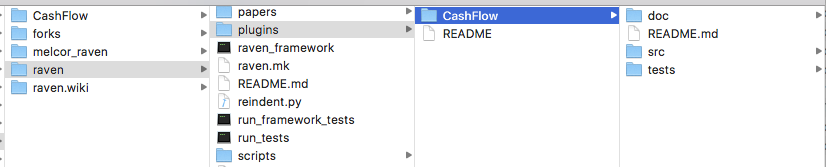
\includegraphics[width=1.0\textwidth]{pics/plugins_location.png}
\caption{Plugins Location}
\label{fig:pluginsLocation}
\end{figure}

The  \textit{\textbf{CashFlow}} plug-in is based on the RAVEN plug-in system. This system is aimed to ease the creation
of external models and modules by external developers without the need to deeply know the internal structure
of the RAVEN software. This system is a transparent API for RAVEN external models.
\\The addition of a plugin does not require modifying RAVEN itself. 
Instead, the developer creates a new Python module that is going to be embedded
 in RAVEN at run-time (no need to introduce  hard-coded statements).
 This plugin (CashFlow for instance) needs to be placed in a folder  located in (see figure~\ref{fig:pluginsLocation}):
\begin{lstlisting}[language=bash]
 path/to/raven/plugins/
\end{lstlisting}
In order to install the CashFlow plugin (if not downloaded by RAVEN submodule system),
 the user can run the script contained in the RAVEN script folder:
\begin{lstlisting}[language=bash]
 python path/to/raven/scripts/install_plugins.py  **directory**/CashFlow
\end{lstlisting}
where  $**directory**$/CashFlow should be replaced with the absolute path to the CashFlow plugin directory.
(e.g. ``path/to/my/plugins/CashFlow''). 

\subsection{CashFlow Structure}
The  \textit{\textbf{CashFlow}} plug-in contains the following methods (API from RAVEN):

\begin{lstlisting}[language=python]
from ExternalModelPluginBase import ExternalModelPluginBase

class CashFlow(ExternalModelPluginBase):
  def run (self, container, Inputs)
  def _readMoreXML(self, container, xmlNode)
  def initialize(self,container, runInfo, inputs)
\end{lstlisting}
In the following sub-sections all the methods are explained.
\subsubsection{Method: \texttt{run}}
\label{subsubsec:runExternalModelPlugin}
\begin{lstlisting}[language=python]
def run (self, container, Inputs)
\end{lstlisting}

In this function, the Cash Flow analysis is coded.
%
The only two attributes this method is going to receive are a Python list of inputs
(the inputs coming from the \texttt{createNewInput} method (see \cite{RAVENuserManual}) and a ``self-like'' object
named ``container''.
%
All the outcomes of the CashFlow module will be stored in the above mentioned ``container'' in order to 
allow RAVEN to collect them.

\subsubsection{Method: \texttt{\_readMoreXML}}
\label{subsubsec:externalReadMoreXMLExternalModelPlugin}
\begin{lstlisting}[language=python]
def _readMoreXML(self, container, xmlNode)
\end{lstlisting}
In this method, the CashFlow input is read and made available to the plug-in and RAVEN.
%
The read information are stored in the ``self-like'' object ``container''
 in order to be available to all the other methods, specifically the  \textbf{run} and  \textbf{initialize} methods. 
%
The method receives from RAVEN an attribute of type ``xml.etree.ElementTree'',
containing all the sub-nodes and attribute of the XML block \xmlNode{ExternalModel}.
%

Example XML:
\begin{lstlisting}[style=XML,morekeywords={subType,ModuleToLoad}]
<CashFlow name="CAPEX" driver="Plant_capacity" tax="false" inflation="none">
  <alpha> -4000000000
  0.0 0.0 0.0 0.0 0.0 0.0 0.0 0.0 0.0 0.0
  0.0 0.0 0.0 0.0 0.0 0.0 0.0 0.0 0.0 0.0</alpha>
  <reference>1000000000</reference>
  <X>0.64</X> 
</CashFlow>
\end{lstlisting}

\subsubsection{Method: \texttt{initialize}}
\label{subsubsec:externalInitializeExternalModelPlugin}
\begin{lstlisting}[language=python]
def initialize(self, container, runInfo, inputs)
\end{lstlisting}

The \textbf{initialize} method is implemented  to initialize the Cash Flow analysis based on
the current RAVEN status and CashFlow input file (The XML input file).
%
 \\Indeed, RAVEN is going to call this method at the initialization stage of each ``Step'' (see section \cite{RAVENuserManual}).
%
RAVEN will communicate, thorough a set of method attributes, all the information
that are needed to perform an initialization:
\begin{itemize}
  \item runInfo, a dictionary containing information regarding how the
  calculation is set up (e.g. number of processors, etc.).
  %
  It contains the following attributes:
  \begin{itemize}
    \item \texttt{DefaultInputFile} -- default input file to use
    \item \texttt{SimulationFiles} -- the xml input file
    \item \texttt{ScriptDir} -- the location of the pbs script interfaces
    \item \texttt{FrameworkDir} -- the directory where the framework is located
    \item \texttt{WorkingDir} -- the directory where the framework should be
    running
    \item \texttt{TempWorkingDir} -- the temporary directory where a simulation
    step is run
    \item \texttt{NumMPI} -- the number of mpi process by run
    \item \texttt{NumThreads} -- number of threads by run
    \item \texttt{numProcByRun} -- total number of core used by one run (number
    of threads by number of mpi)
    \item \texttt{batchSize} -- number of contemporaneous runs
    \item \texttt{ParallelCommand} -- the command that should be used to submit
    jobs in parallel (mpi)
    \item \texttt{numNode} -- number of nodes
    \item \texttt{procByNode} -- number of processors by node
    \item \texttt{totalNumCoresUsed} -- total number of cores used by driver
    \item \texttt{queueingSoftware} -- queueing software name
    \item \texttt{stepName} -- the name of the step currently running
    \item \texttt{precommand} -- added to the front of the command that is run
    \item \texttt{postcommand} -- added after the command that is run
    \item \texttt{delSucLogFiles} -- if a simulation (code run) has not failed,
    delete the relative log file (if True)
    \item \texttt{deleteOutExtension} -- if a simulation (code run) has not
    failed, delete the relative output files with the listed extension (comma
    separated list, for example: `e,r,txt')
    \item \texttt{mode} -- running mode, curently the only mode supported is
      mpi (but custom modes can be created)
    \item \textit{expectedTime} -- how long the complete input is expected to
    run
    \item \textit{logfileBuffer} -- logfile buffer size in bytes
  \end{itemize}
  \item inputs, a list of all the inputs that have been specified in the
  ``Step'' using this model.
  %
\end{itemize}





\subsection{Data Design and Control}
The data transfer in the \textbf{\textit{TEAL}}  plug-in is fully standardized via the API for External Model Plug-In, via
Python dictionaries.
\\The documentation of this  API is reported in the RAVEN user manual (\cite{RAVENuserManual})

\subsection{Human-Machine Interface Design} 
 There are no human system integration requirements associated with this software.

 \subsection{Security Structure} 
The software is accessible to the open-source community (Apache License, Version 2.0). No restrictions for downloading or redistributing is applicable.

% THIS SECTION SHOULD BE REPLACED WITH THE ONE ABOVE ONCE IT GOES OPEN-SOURCE

%The software is accessible via GITHUB to licensed users and is publicaly available.

 \section{REQUIREMENTS CROSS-REFERENCE} 
The requirements are detailed in SPC-2895, ``TEAL Software Requirements Specification (SRS) and Traceability Matrix''.




    % ---------------------------------------------------------------------- %
    % References
    %

\addcontentsline{toc}{section}{References}
\bibliographystyle{ieeetr}
\bibliography{cash_flow_software_design_description}

\section*{Document Version Information}

f8a46c15f16e3c95179586e647f807b684fb36d3 Paul W. Talbot\\Tue, 29 Sep 2020 13:20:59 -0600


\end{document}
